\documentclass[a4paper, 12pt]{article}

\usepackage{geometry}
\geometry{left=2cm, right=2cm, top=2cm, bottom=2cm}
\usepackage{wrapfig}
\usepackage{cmap}
\usepackage{mathtext} 
\usepackage[T2A]{fontenc}
\usepackage[utf8]{inputenc}
\usepackage[english,russian]{babel}	

\usepackage{amsfonts,amssymb,amsthm,mathtools}
\usepackage{amsmath}
\usepackage{icomma} 

\usepackage{graphicx} 
\graphicspath{{picturies/}}
\usepackage{wrapfig}

\usepackage{array,tabularx,tabulary,booktabs}
\usepackage{longtable}
\usepackage{multirow}

\usepackage{caption}
\captionsetup{labelsep=period}

\renewcommand{\phi}{\varphi}
\newcommand{\eps}{\varepsilon}
\newcommand{\parag}[1]{\paragraph*{#1:}}
\newcommand{\mysec}[1]{\begin{center}\section*{#1}\end{center}}

\author{Радькин Кирилл Б01-005}
\title{3.6.1 Спектральный анализ электрических сигналов}
\date{19.11.21}

\graphicspath{{pictures/}}

\begin{document}
    \maketitle

    \parag{Цель работы} изучение спектрального состава периодических электрических сигналов

    \parag{В работе используются} анализатор спектра, генератор прямоугольных импульсов, генератор сигналов специальной формы, осциллограф
    \\\\
    В работе изучается спектральный состав периодических сигналов различной формы: последовательности прямоугольных импульсов, последовательности цугов и амплитудно-модулированных гармонических колебаний. Спектры этих сигналов наблюдаются с помощью промышленного анализатора спектра и сравниваются с расчитанными теоретически.

    \paragraph*{Принцип работы спектроанализатора.} 
    Для исследования спектров в работе используется гетеродинный анализатор спектра типа СК4-56. Упрощенная структурная схема, поясняющая последовательный супергетеродинный метод спектрального анализа внешнего сигнала, изображена на рис.~1.

    \begin{figure}[!h]
        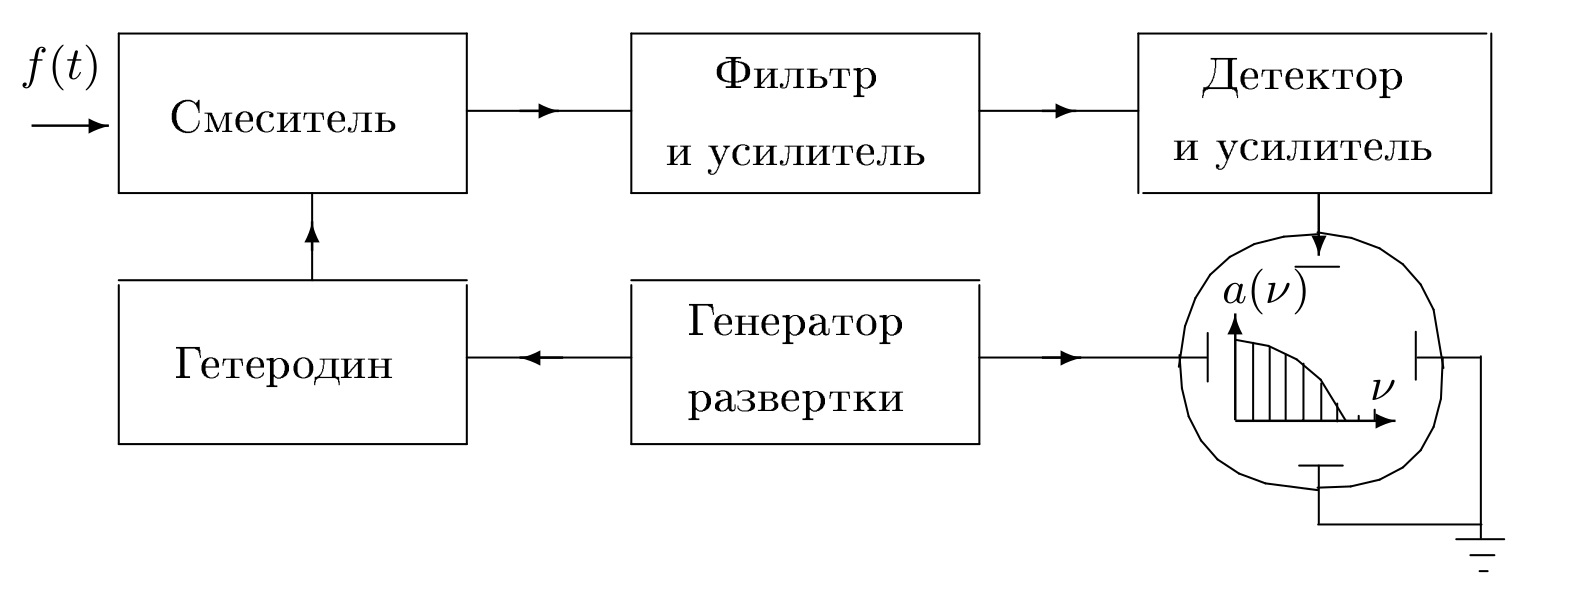
\includegraphics[scale=0.3]{pic1.png}
        \caption{структурная схема анализатора спектра}
    \end{figure}

    \mysec{A. Исследование спектра периодической последовательности прямоугольных импульсов}
    
    \paragraph*{Экспериментальная установка.}
    Схема для исследования спектра периодической последовательности импульсов представлена на рис. 2.

    \begin{figure}
        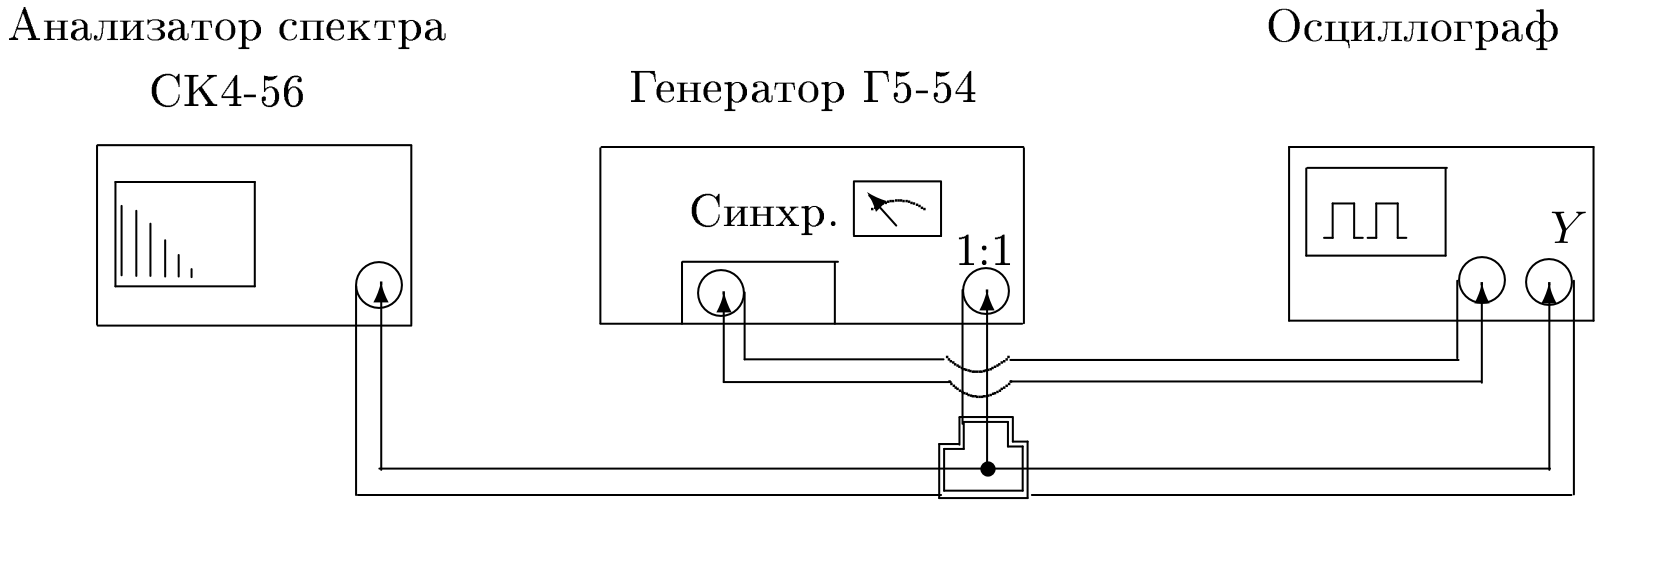
\includegraphics[scale=0.3]{pic2.png}
        \caption{Схема для исследования спектра периодической последовательности прямоугольных импульсов}
    \end{figure}

    В наблюдаемом спектре отсутствует информация об амплитуде нулевой гармоники, т.~е. о величине постоянной составляющей; ее местоположение (начало отсчета шкалы частот) отмечено небольшим выбросом.

    \paragraph*{Задание.}
    
    \begin{enumerate}
        \item Соберем схему согласно рис.~2 и подготовим приборы к работе, следуя техническому описанию, расположенному на установке.

        \item Установим на анализаторе спектра режим работы с однократной разверткой и получим на экране спектр импульсов с параметрами (частотный масштаб $m_x = 5$ кГц/дел.):

        \begin{itemize}
            \item $f_{повт} = 1 \text{ кГц, } \tau = 50 \text{ мкс, }$
            
            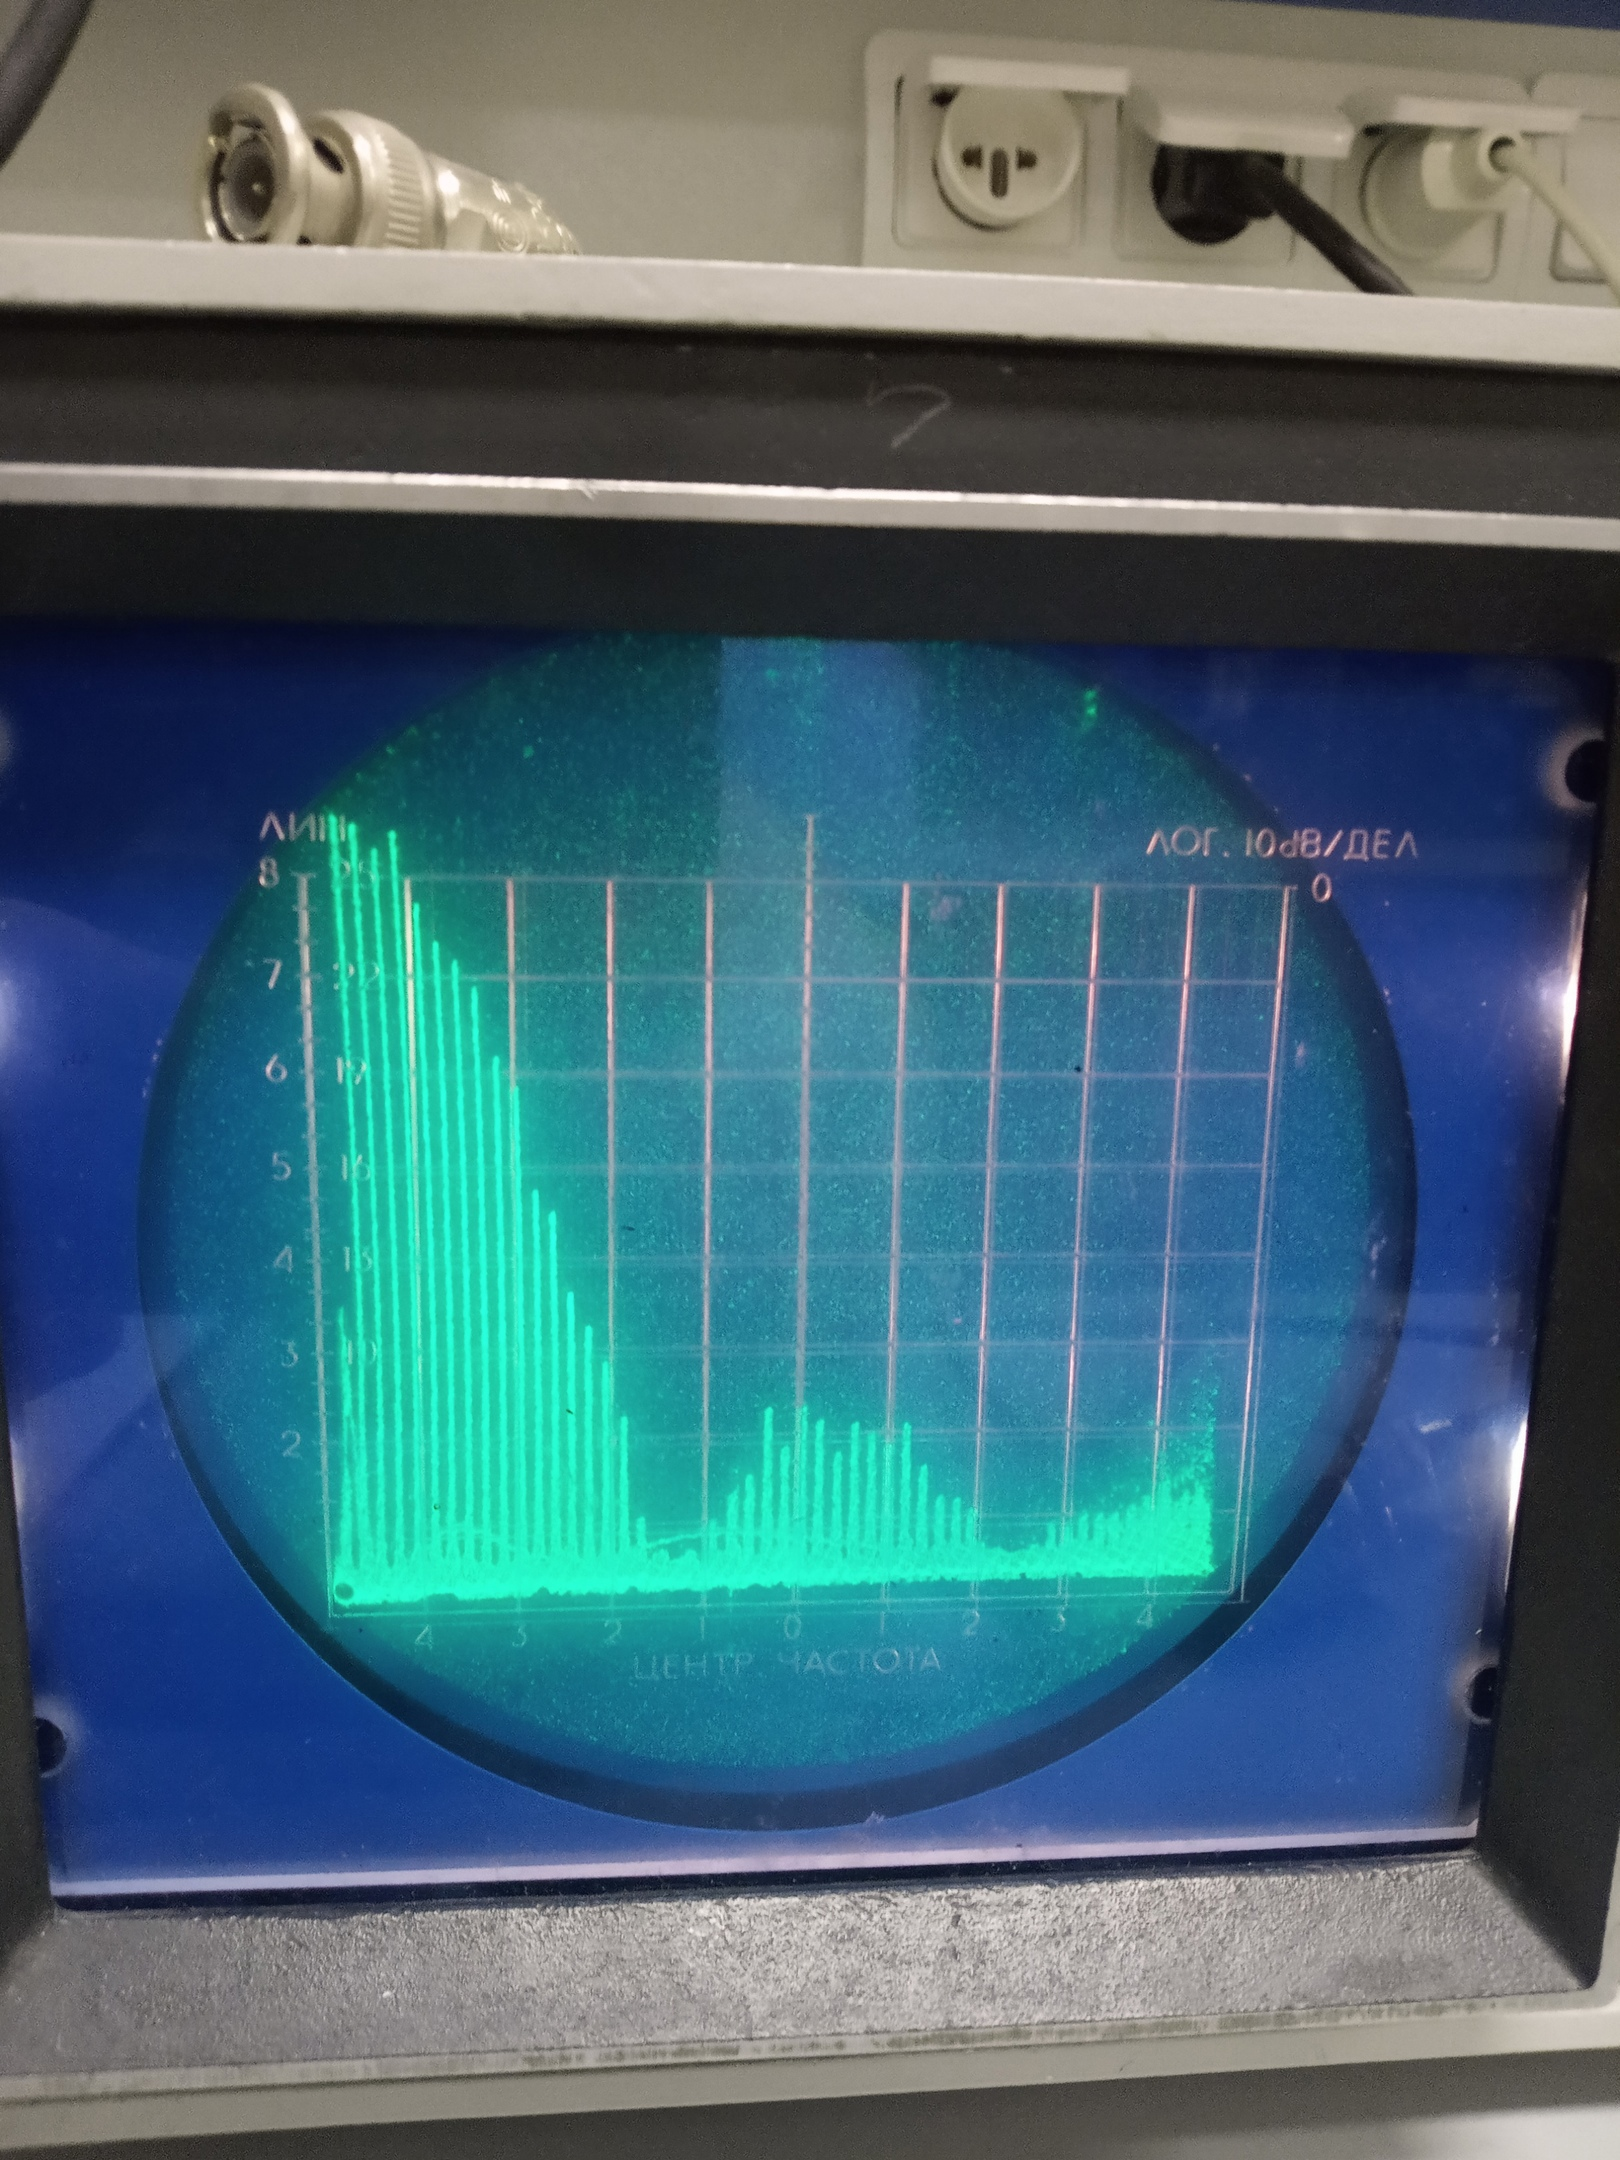
\includegraphics[scale=0.17]{sp1.jpg}

            \item $f_{повт} = 1 \text{ кГц, } \tau = 100 \text{ мкс, }$
            
            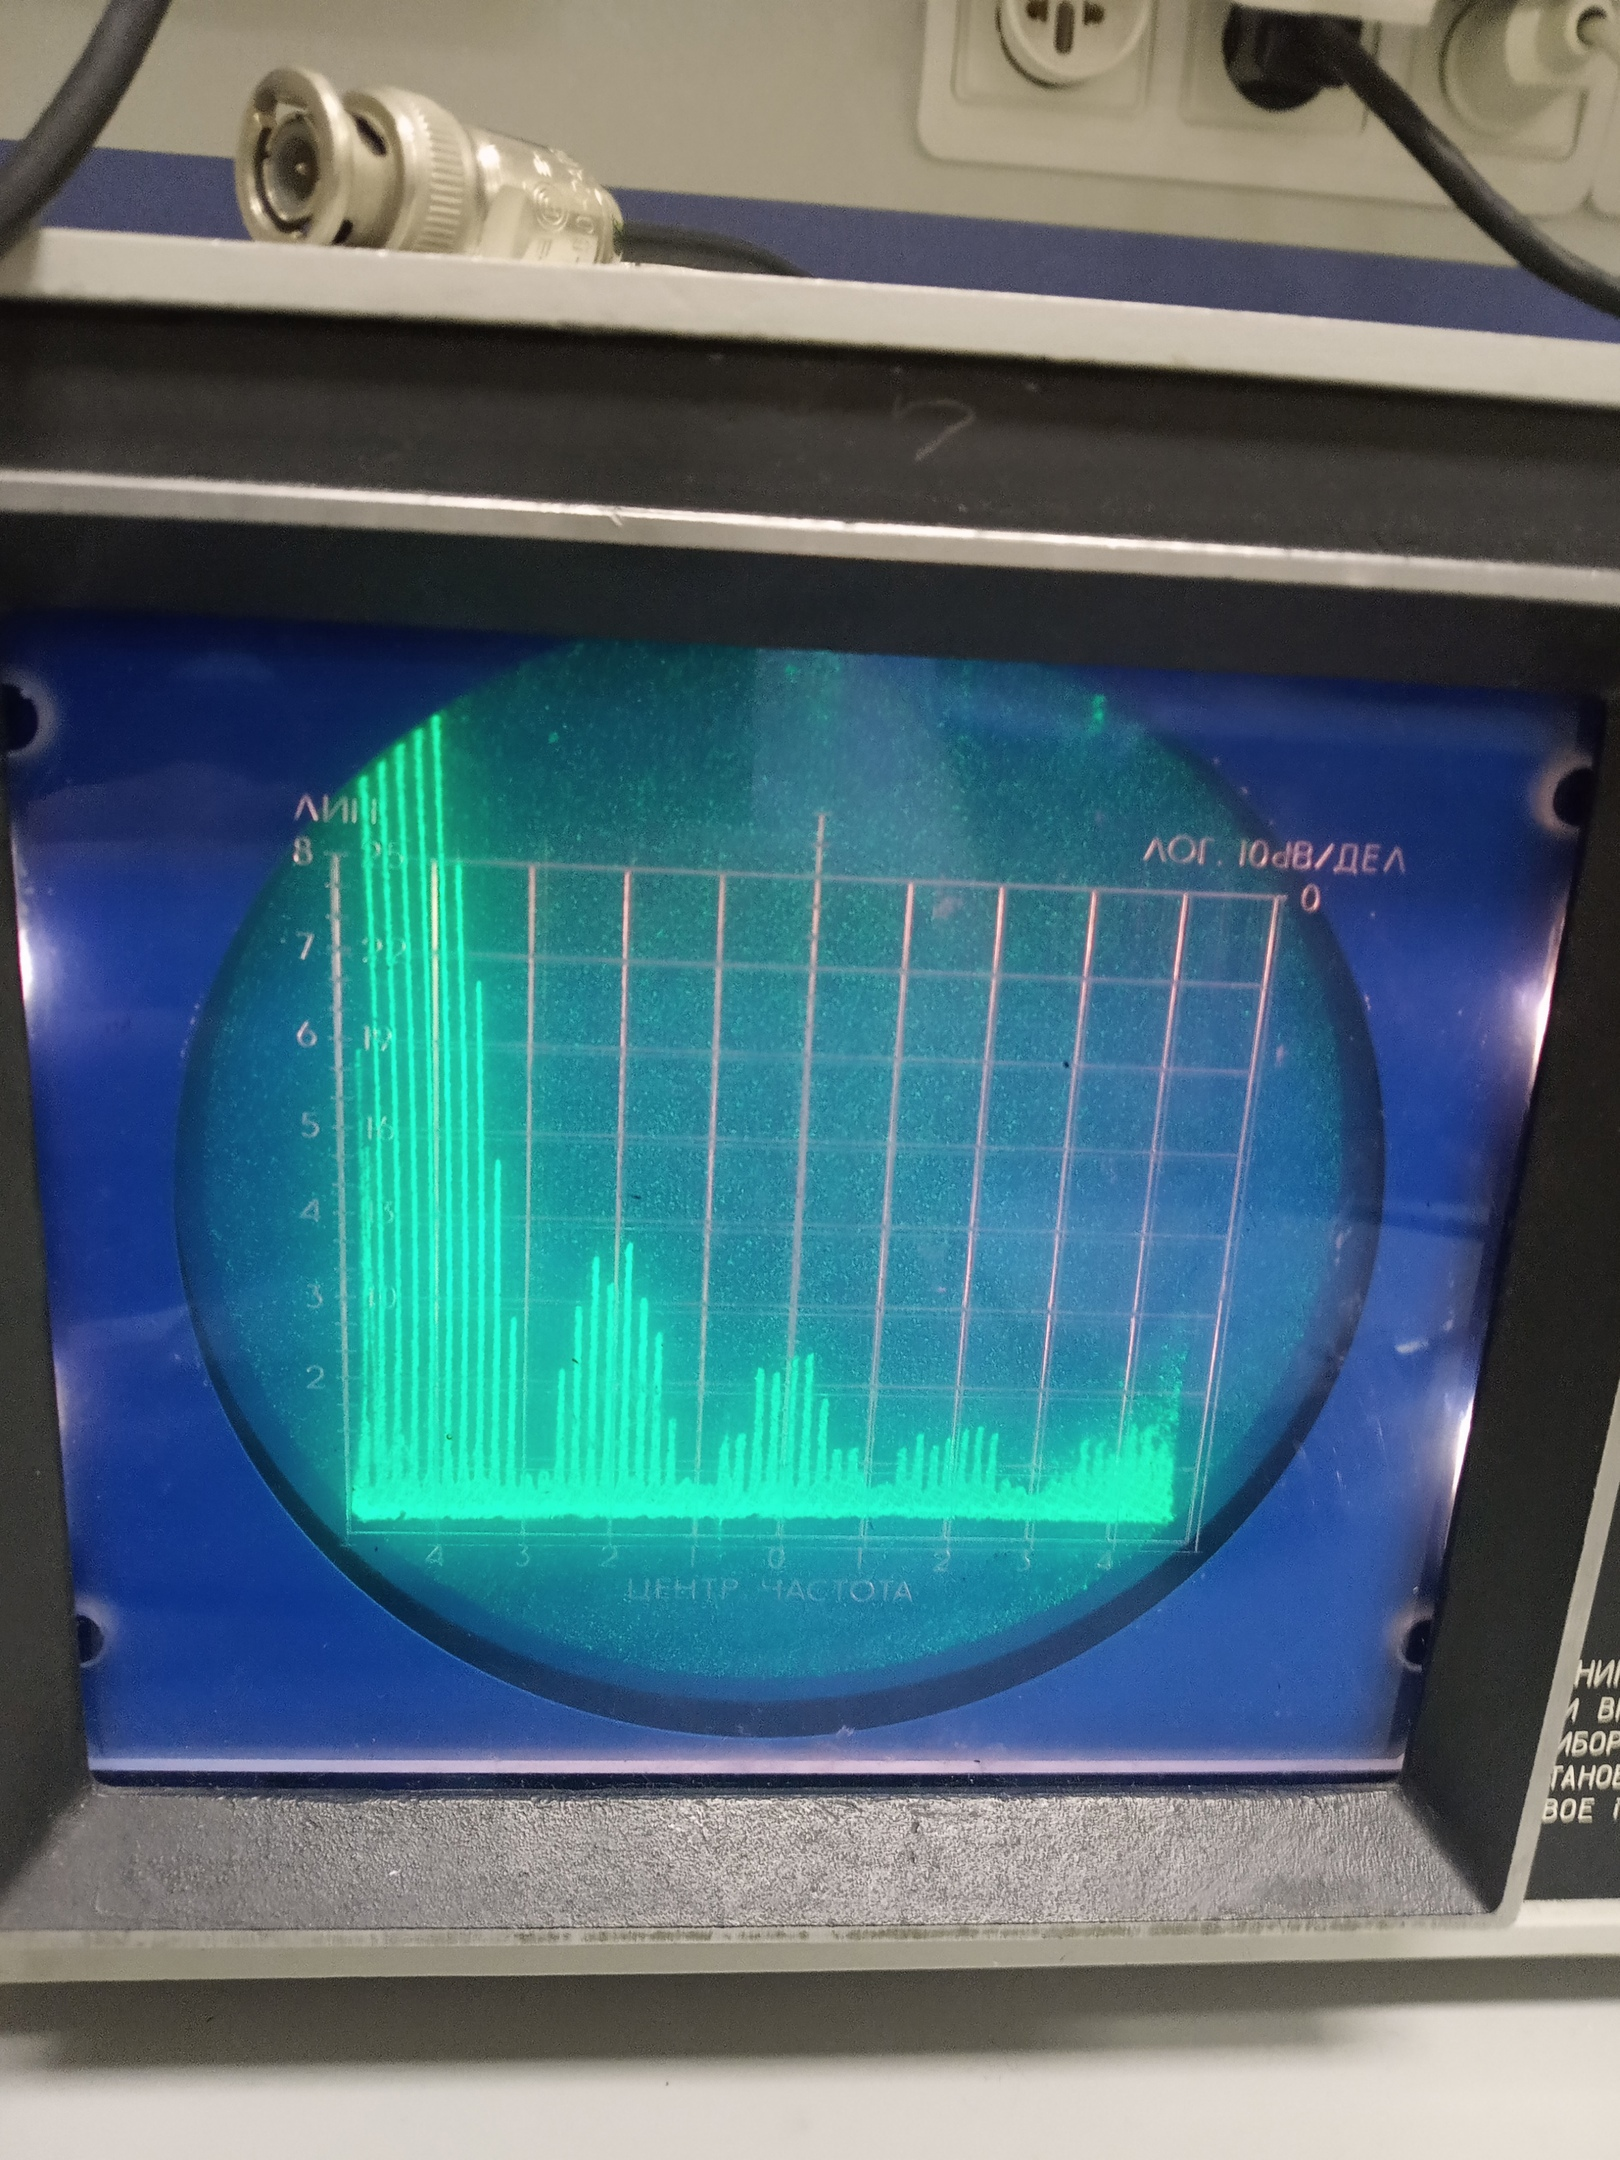
\includegraphics[scale=0.15]{sp2.jpg}

            \item $f_{повт} = 2 \text{ кГц, } \tau = 50 \text{ мкс, }$
            
            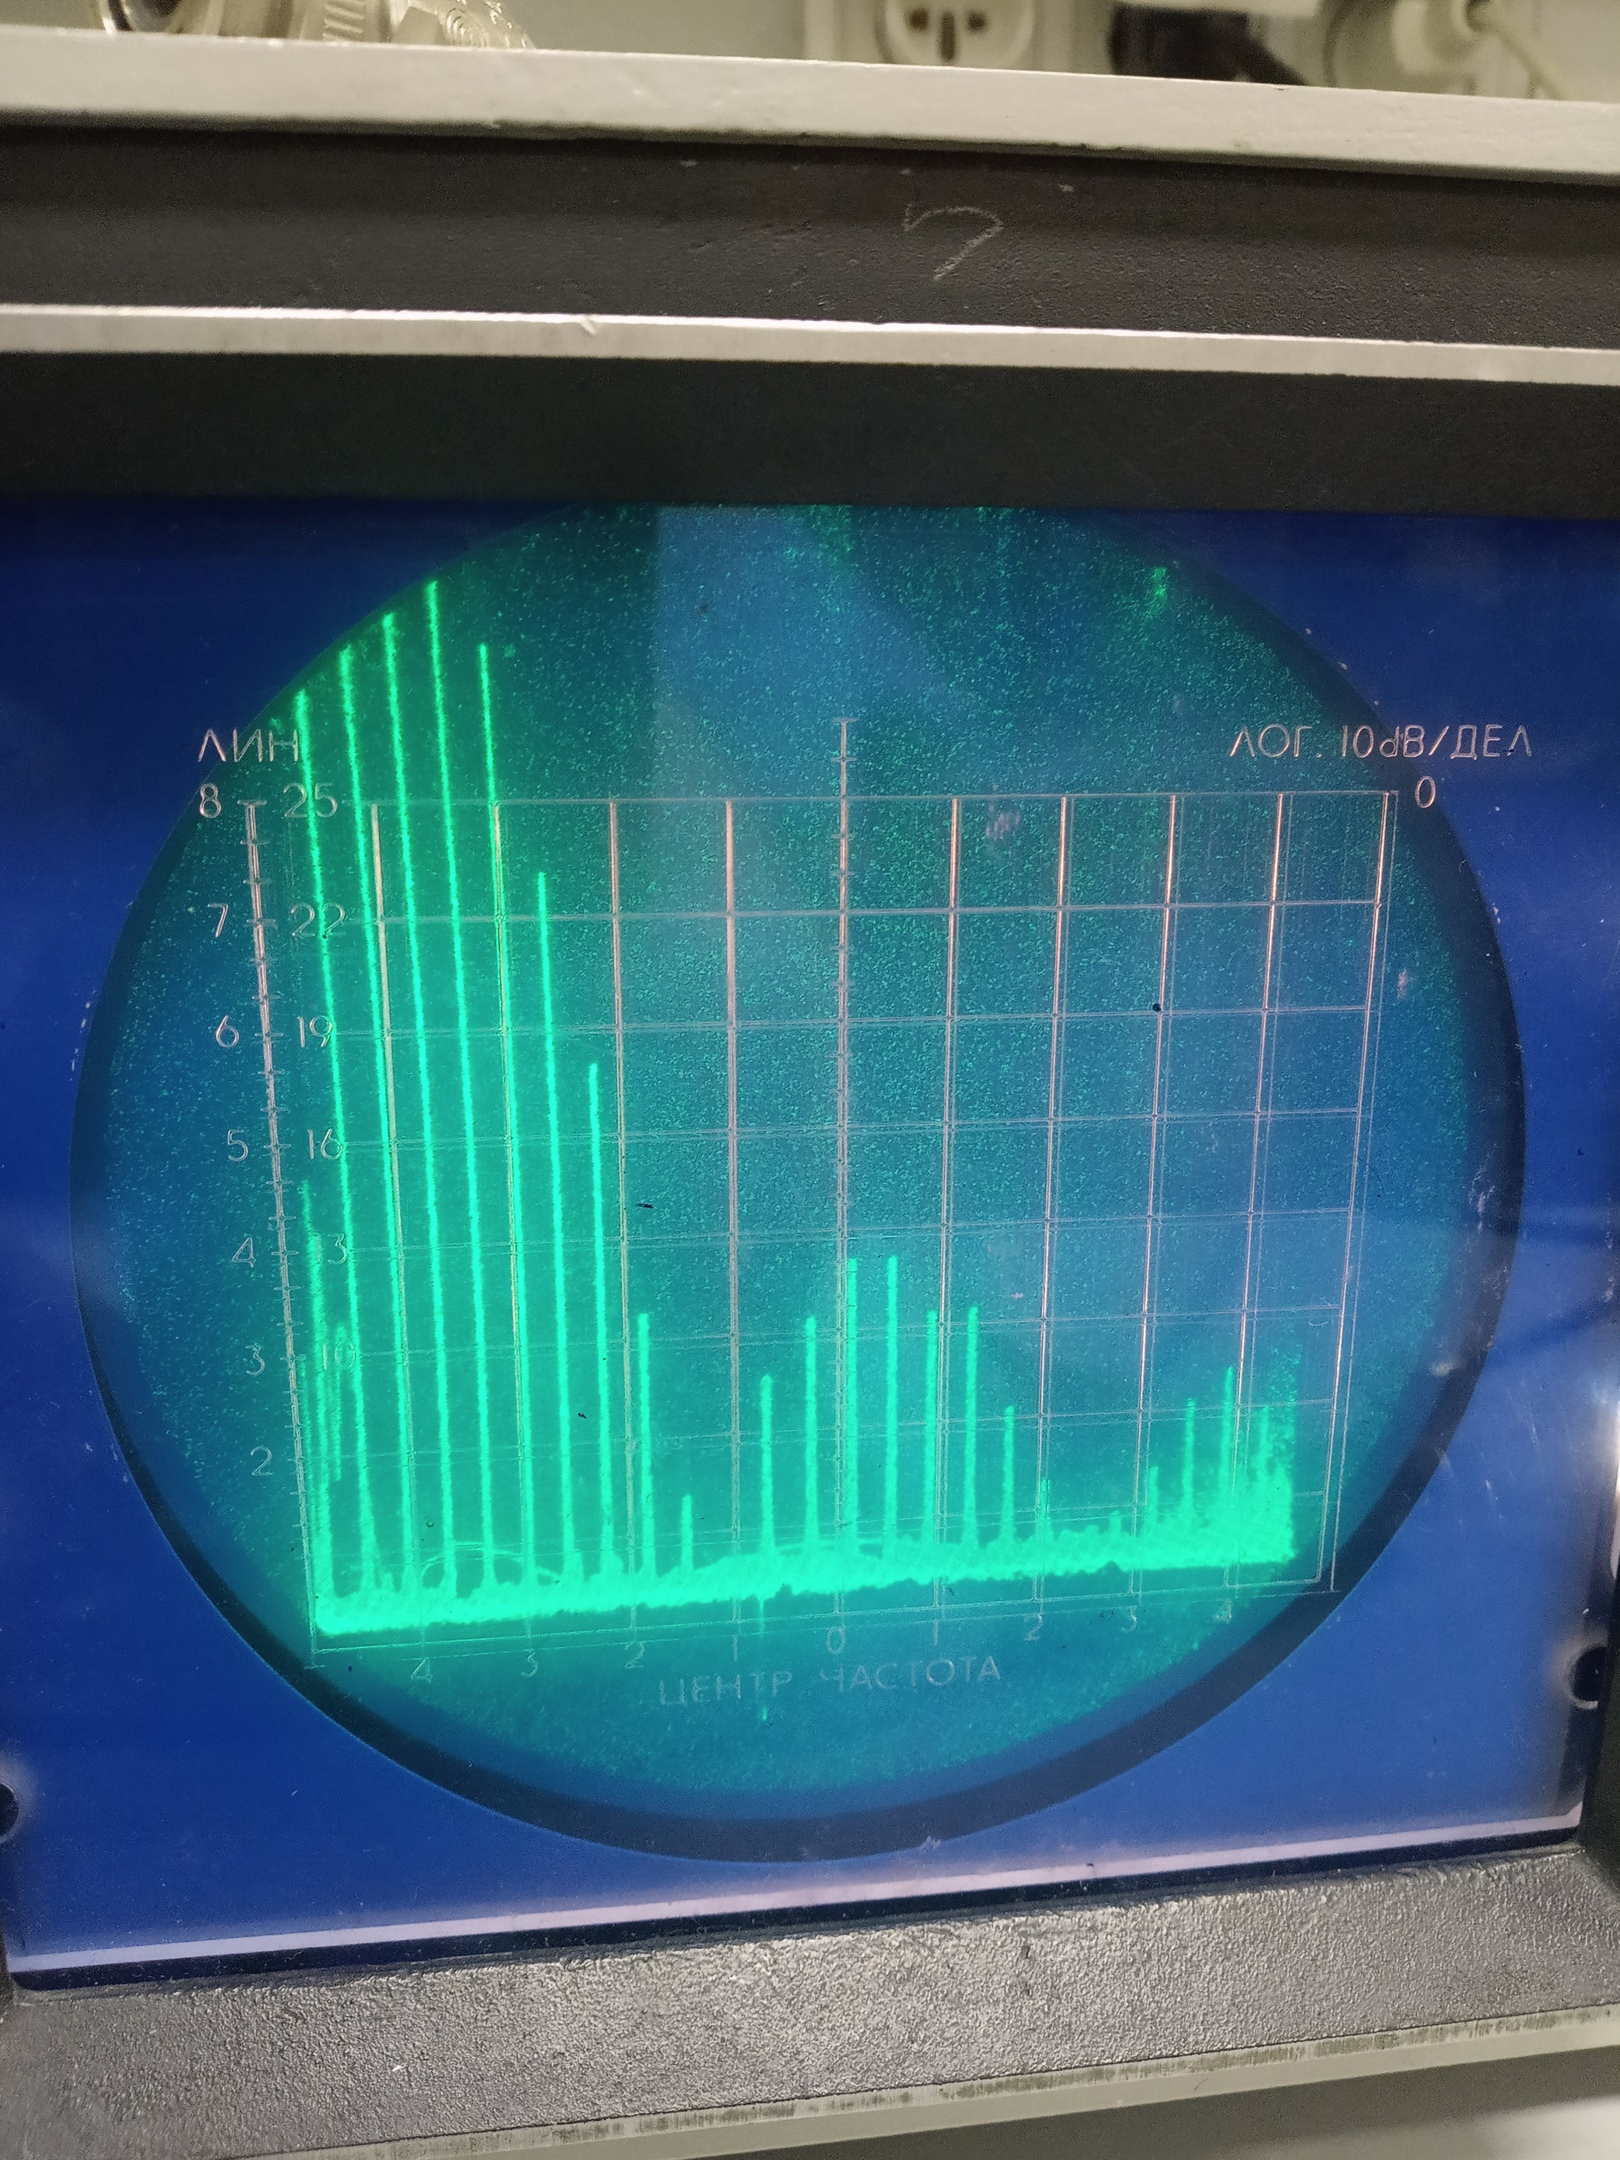
\includegraphics[scale=0.15]{sp3.jpg}
        \end{itemize}

        \item Проведем измерения зависимости ширины спектра от длительности импульса при увеличении $\tau$ от 25 до 200 мкс (1 деление для $\Delta \nu$~---~5 кГц).

        \begin{tabular}{|c|c|c|c|c|c|c|c|c|} \hline
            $\Delta \nu$, дел. & 8 & 4 & 3 & 2 & 1.5 & 1.2 & 1.1 & 0.9 \\ \hline
            $\tau$, мкс & 25 & 50 & 75 & 100 & 125 & 150 & 175 & 200 \\ \hline
        \end{tabular}

        \item Построим график $\Delta \nu \left( 1/\tau \right)$ и по его наклону убедимся, что выполняется соотношение неопределенностей.
            
        \begin{figure}[!h]
            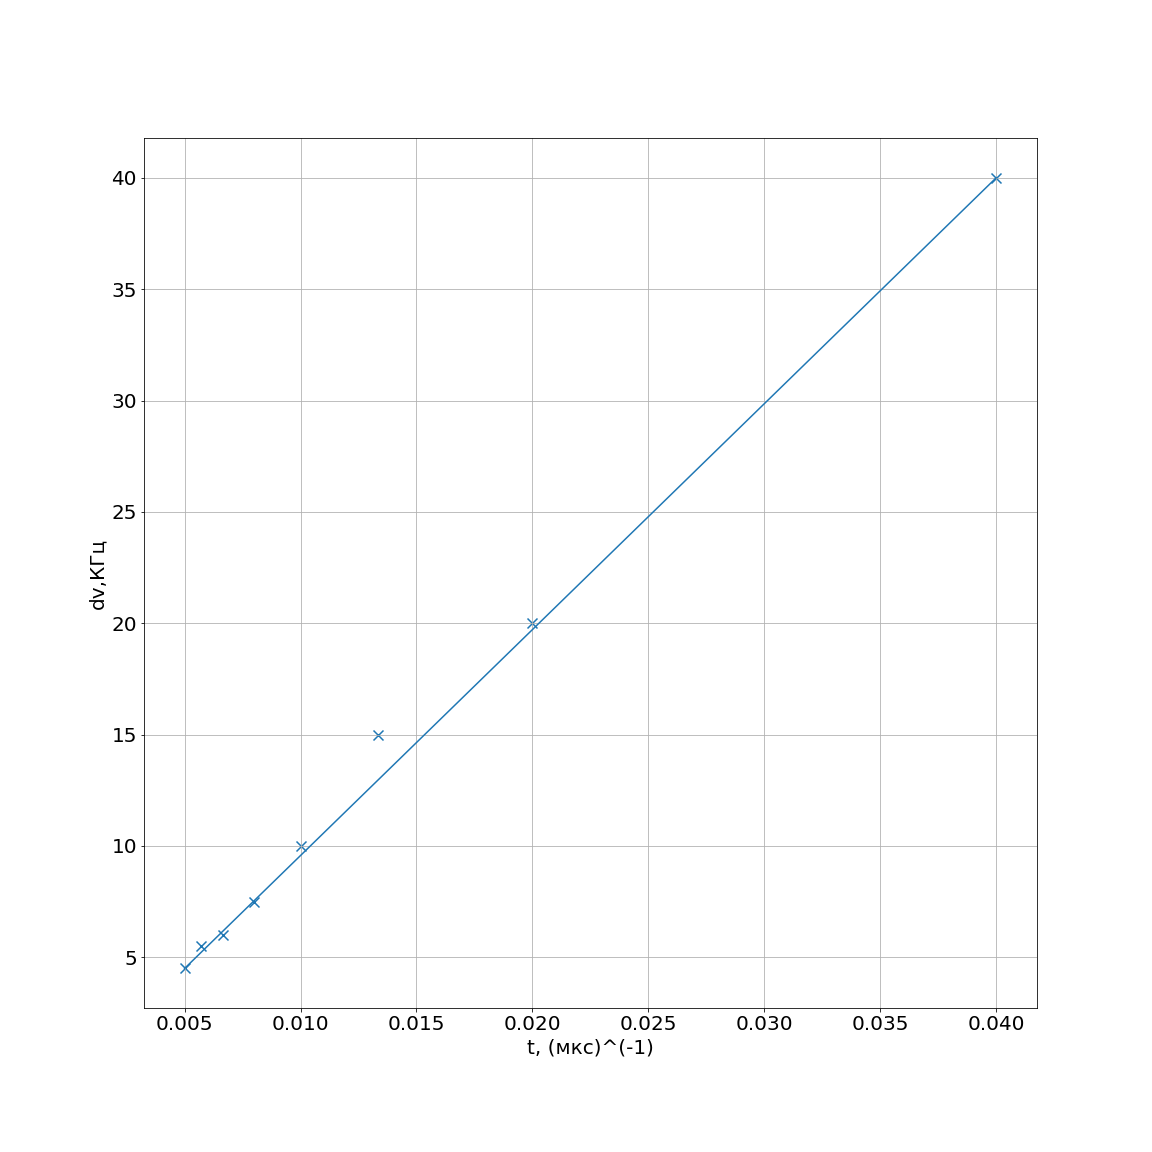
\includegraphics[scale=0.4]{graph1.png}
            \caption{График $\Delta \nu$ от $\tau$}
        \end{figure}

        Из графика: $\Delta \nu \cdot \Delta \tau = 1.09 \pm 0.03$
    \end{enumerate}

    \mysec{Б. Исследование спектра периодической последовательности цугов гармонических колебаний}

    \paragraph*{Экспериментальная установка.} Исследование спектра периодически чередующихся цугов гармонических колебаний проводится по схеме, изображенной на рис.~4. Генератор Г6-34 вырабатывает синусоидоидальные колебания высокой частоты. На вход АМ (амплитудная модуляция) этого генератора подаются прямоугольные импульсы с генератора Г5-54, а на выходе мы получаем высокочастотные модулированные колебания в виде отдельных кусков синусоидоиды~---~цугов. Эти цуги с выхода генератора Г6-34 поступают на вход спектроанализатора и одновременно на вход $Y$ осциллографа. Сигнал синхронизации подается на вход $X$ осциллографа с генератора импульсов.

    \paragraph*{Задание.}

    \begin{enumerate}
        \item Соберем схему, указанную на рис.~4, и подгтовим приборы к работе, руководствуясь техническим описанием.

        \begin{figure}
            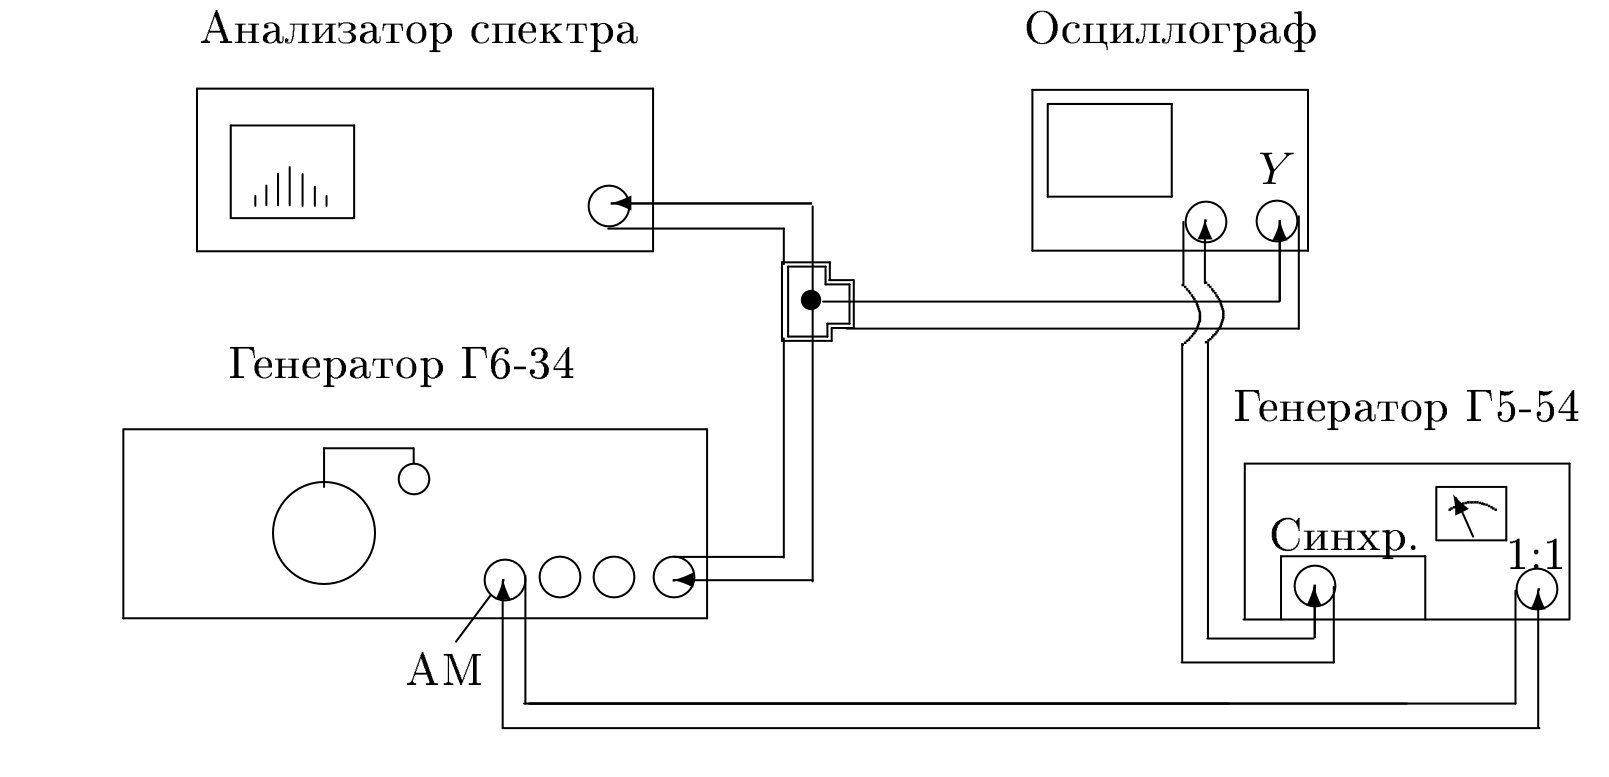
\includegraphics[scale=0.3]{pic3.png}
            \caption{Схема для исследования спектра периодической последовательности цугов высокочастотных колебаний}
        \end{figure}
        
        \item Установим частоту несущей $\nu_0 = 25$ кГц и пронаблюдаем изменения спектра:

        \begin{itemize}
            \item $f_{повт} = 1 \text{ кГц, } \tau = 50 \text{ мкс, } \nu_0 = 25 \text{ кГц, }$
            
            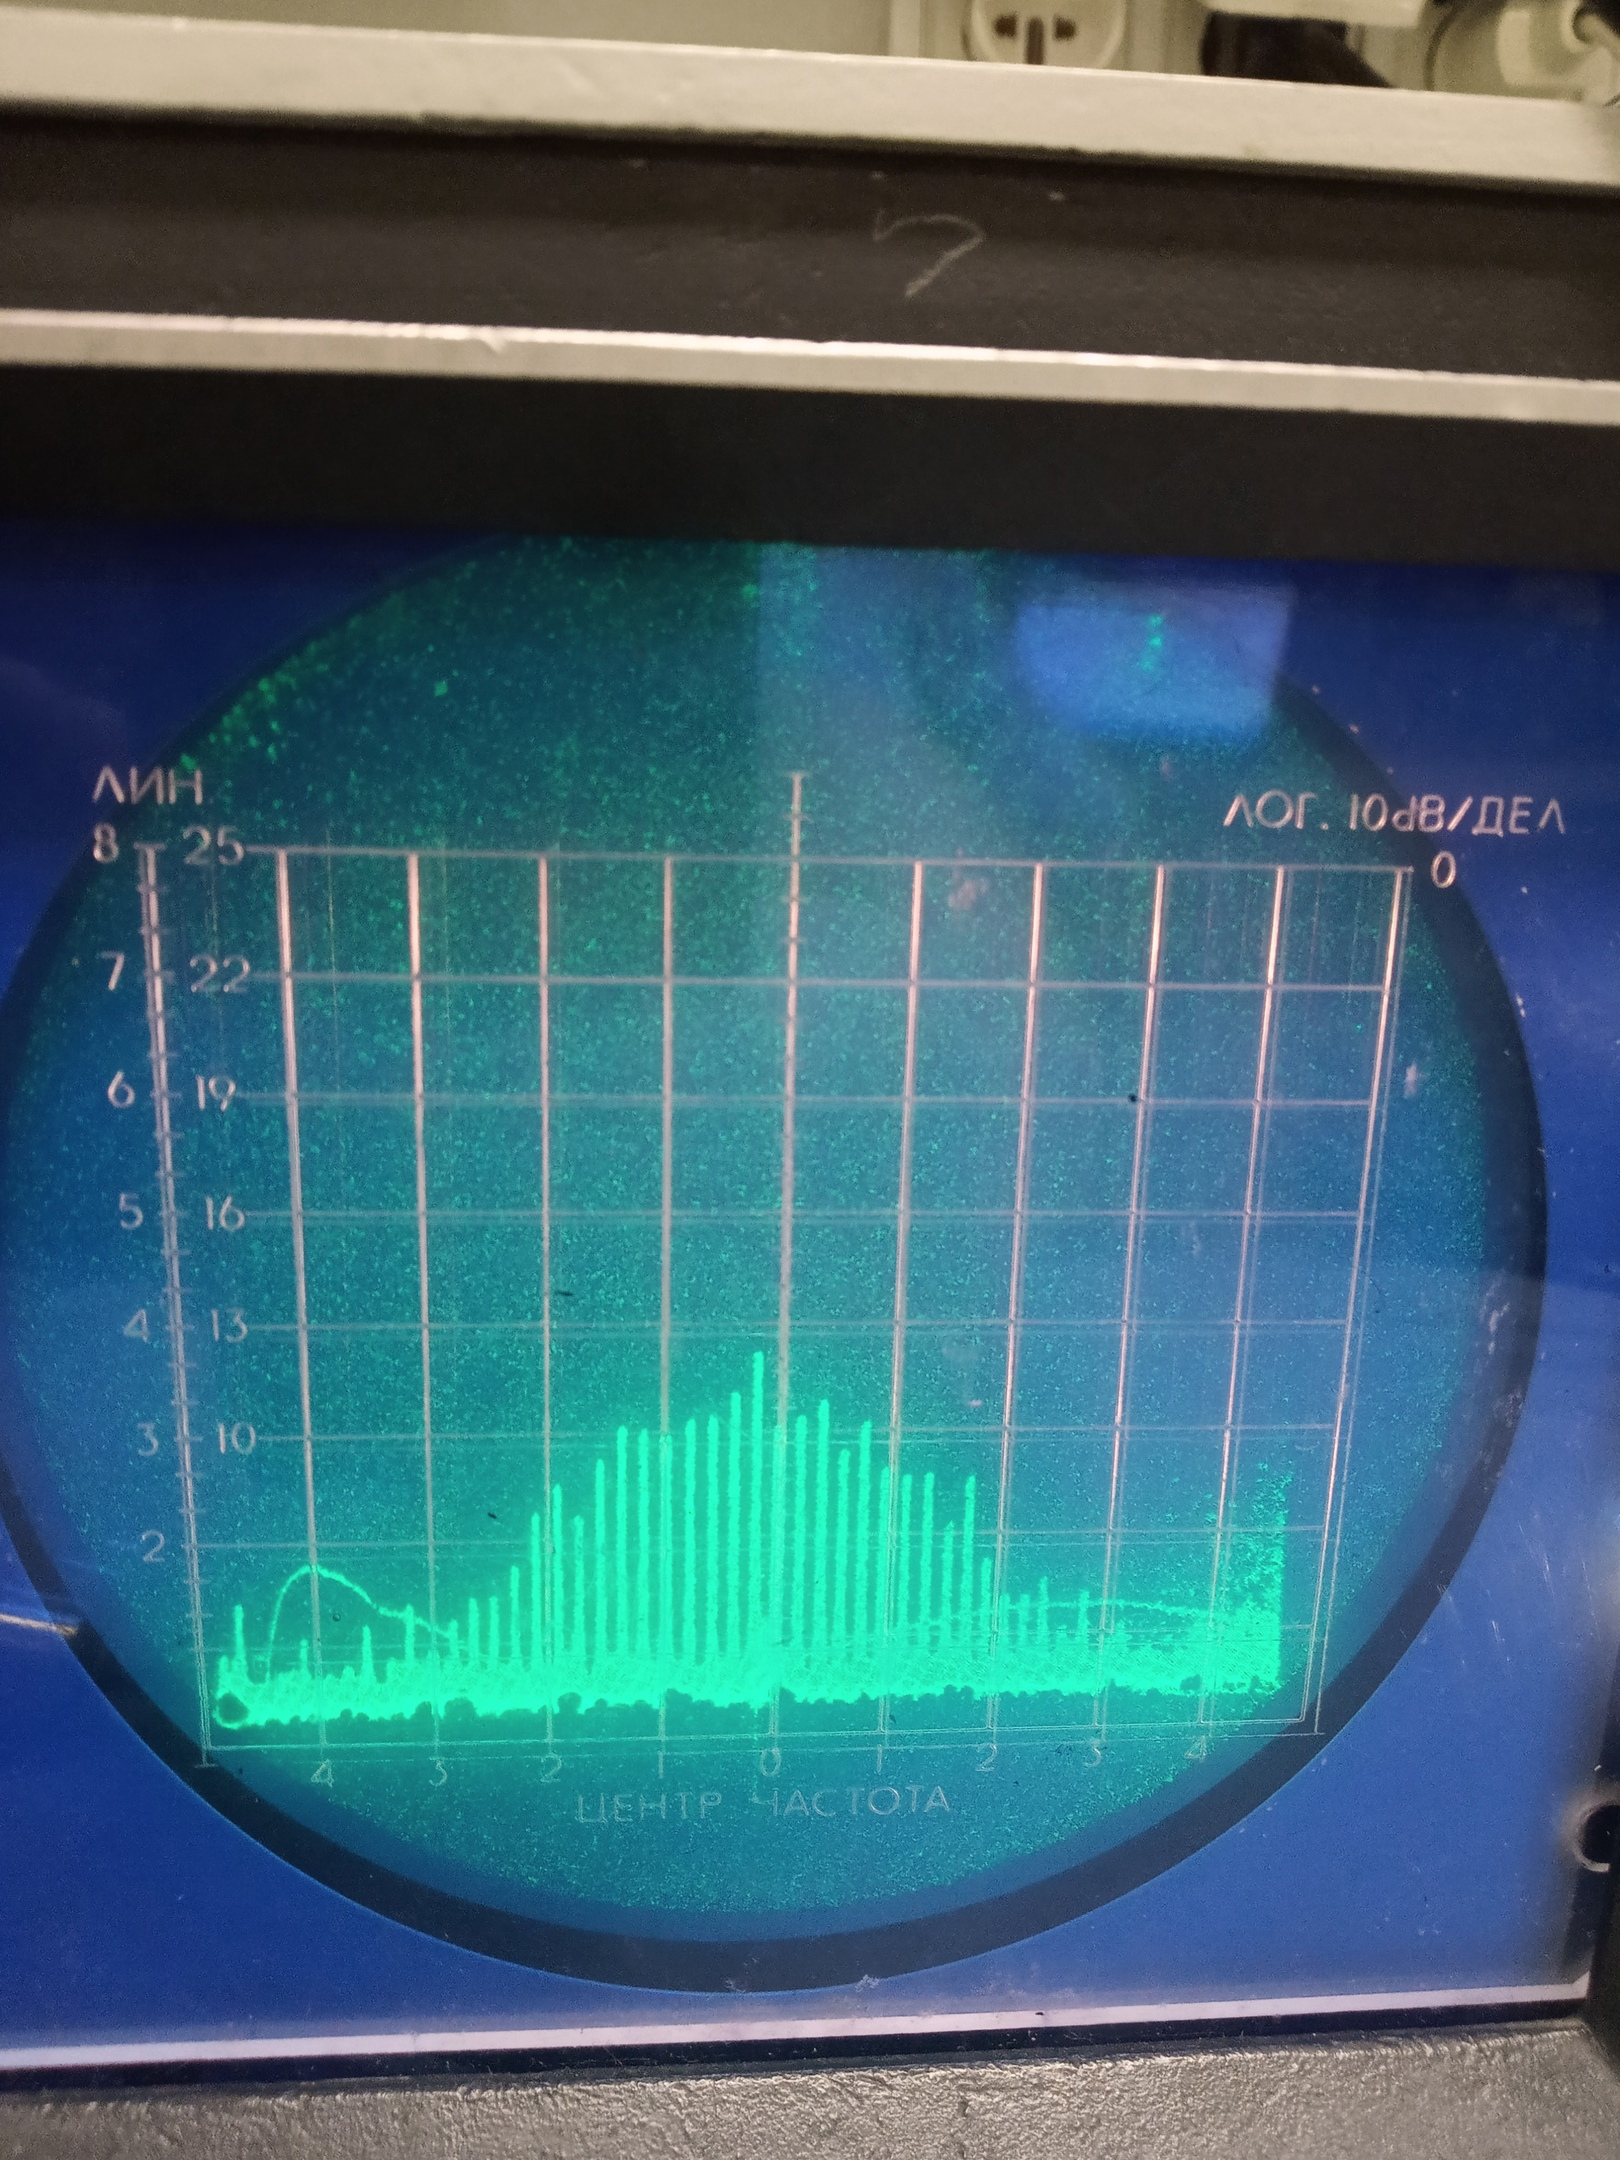
\includegraphics[scale=0.12]{sp4.jpg}

            \item $f_{повт} = 1 \text{ кГц, } \tau = 100 \text{ мкс, } \nu_0 = 25 \text{ кГц, }$

            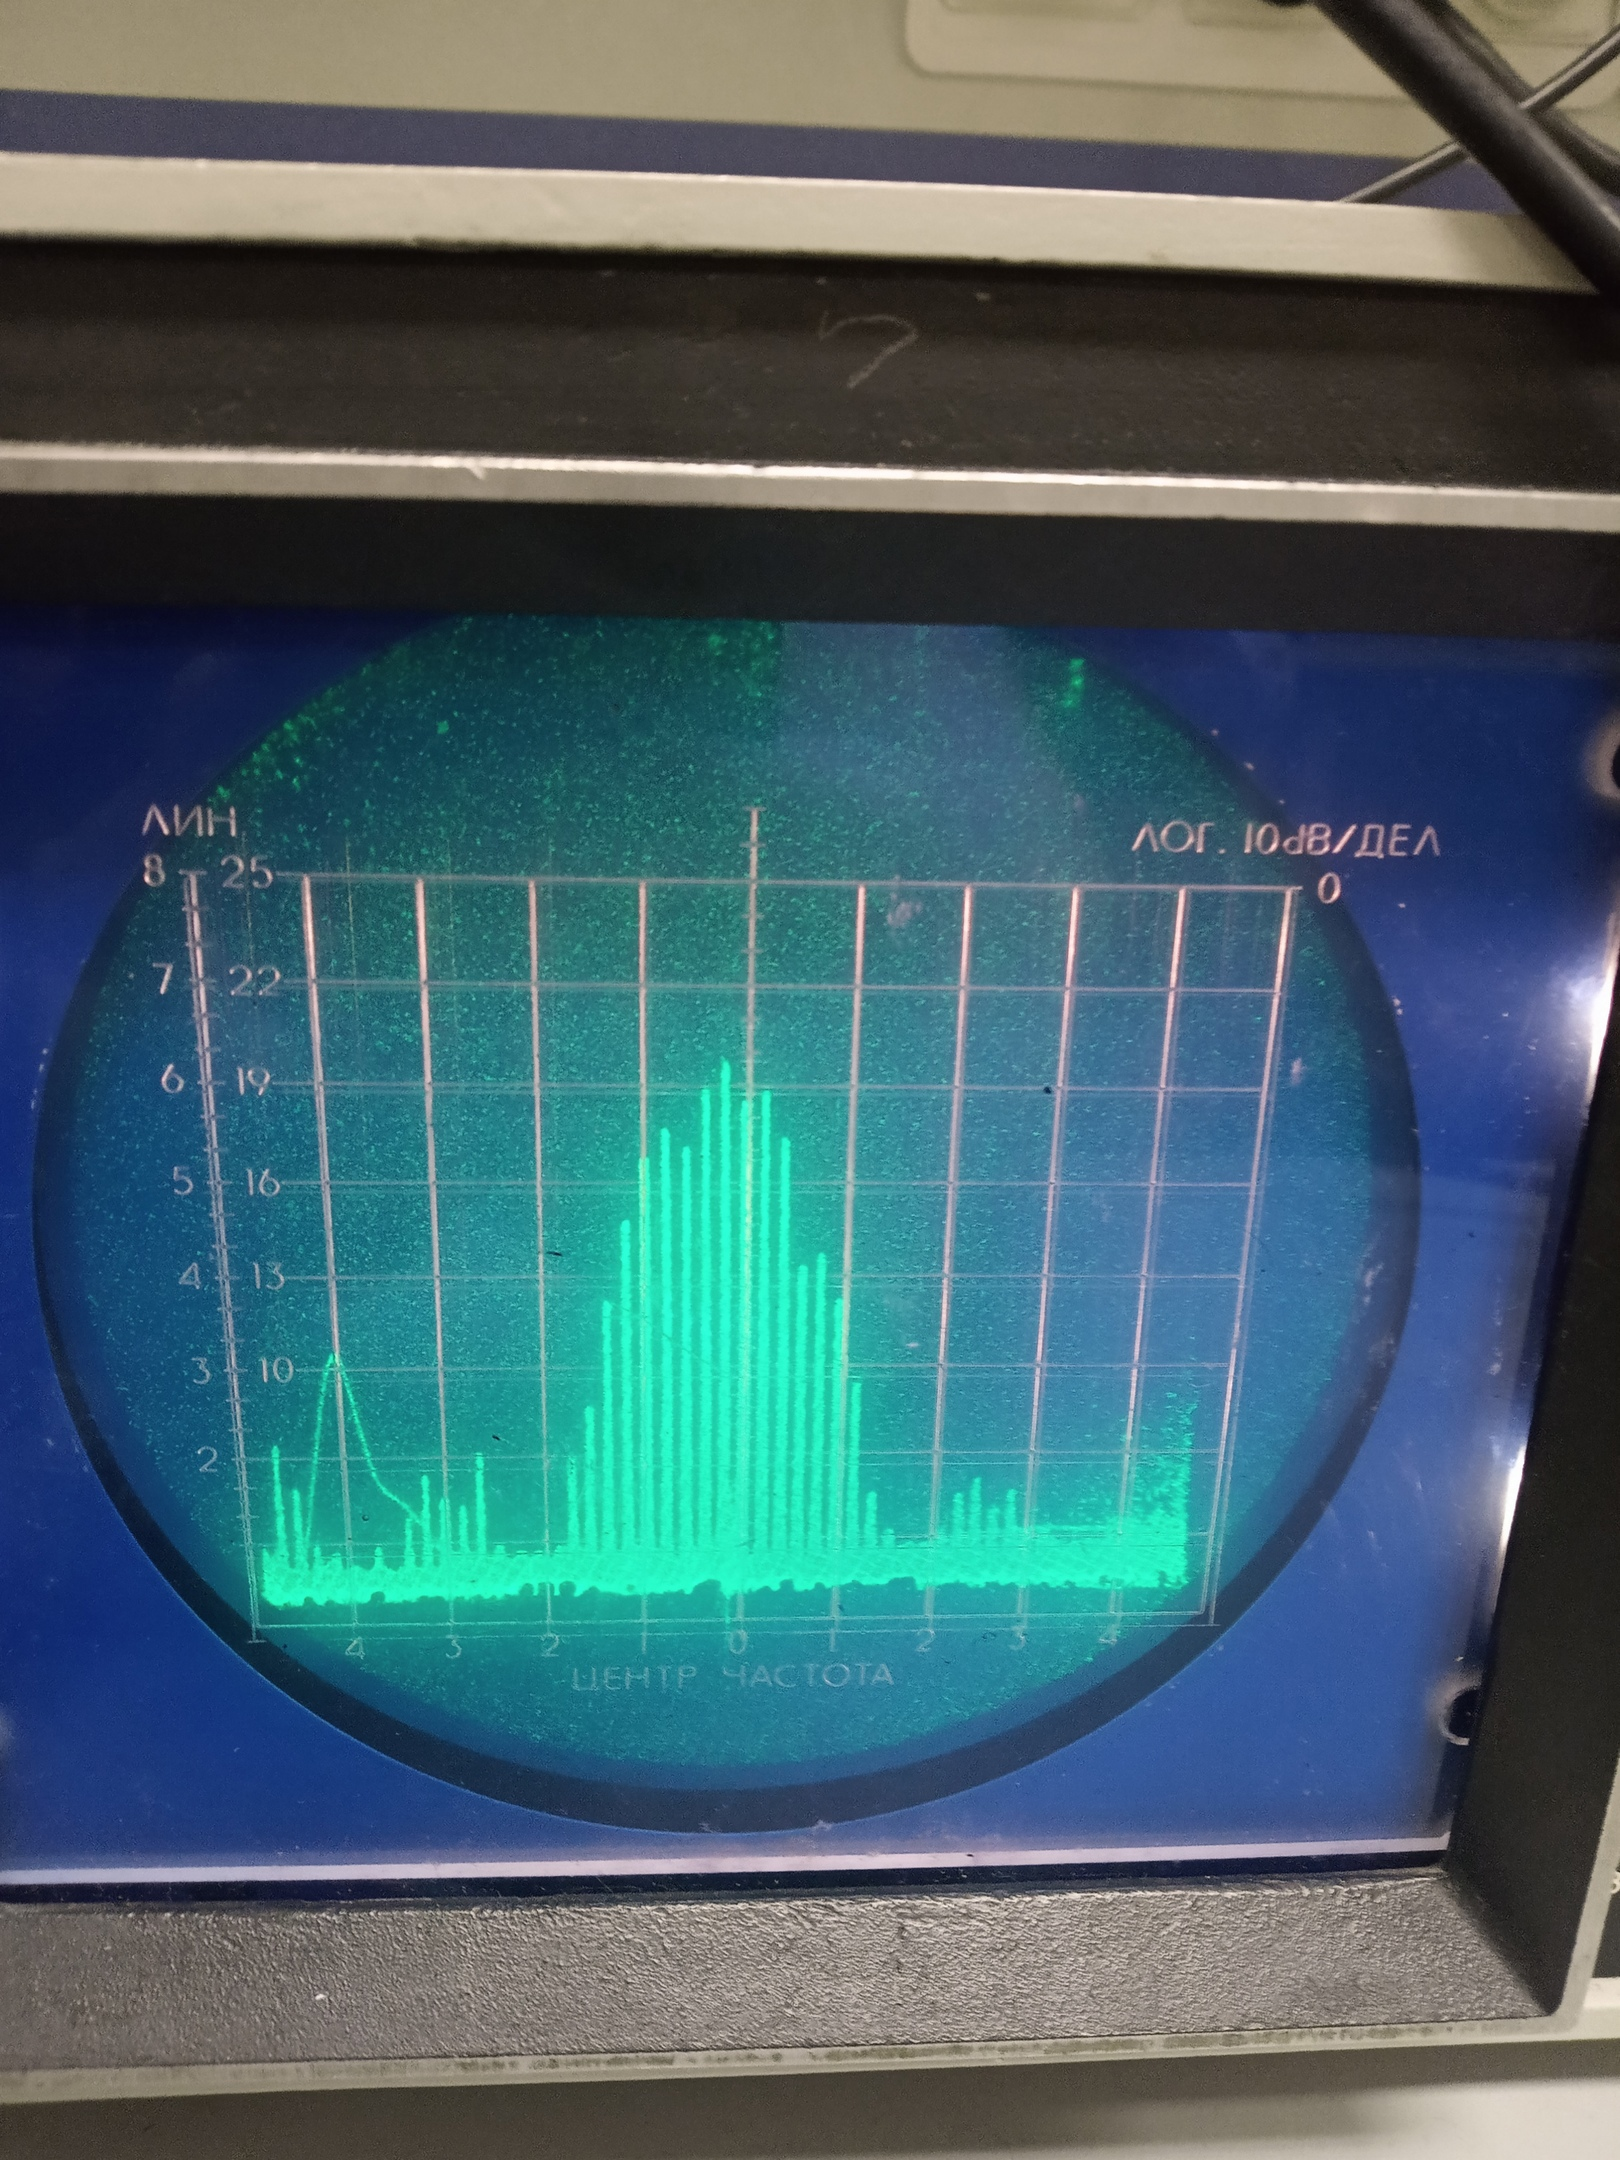
\includegraphics[scale=0.15]{sp5.jpg}

            \item $f_{повт} = 1 \text{ кГц, } \tau = 50 \text{ мкс, } \nu_0 = 10 \text{ кГц, }$
            
            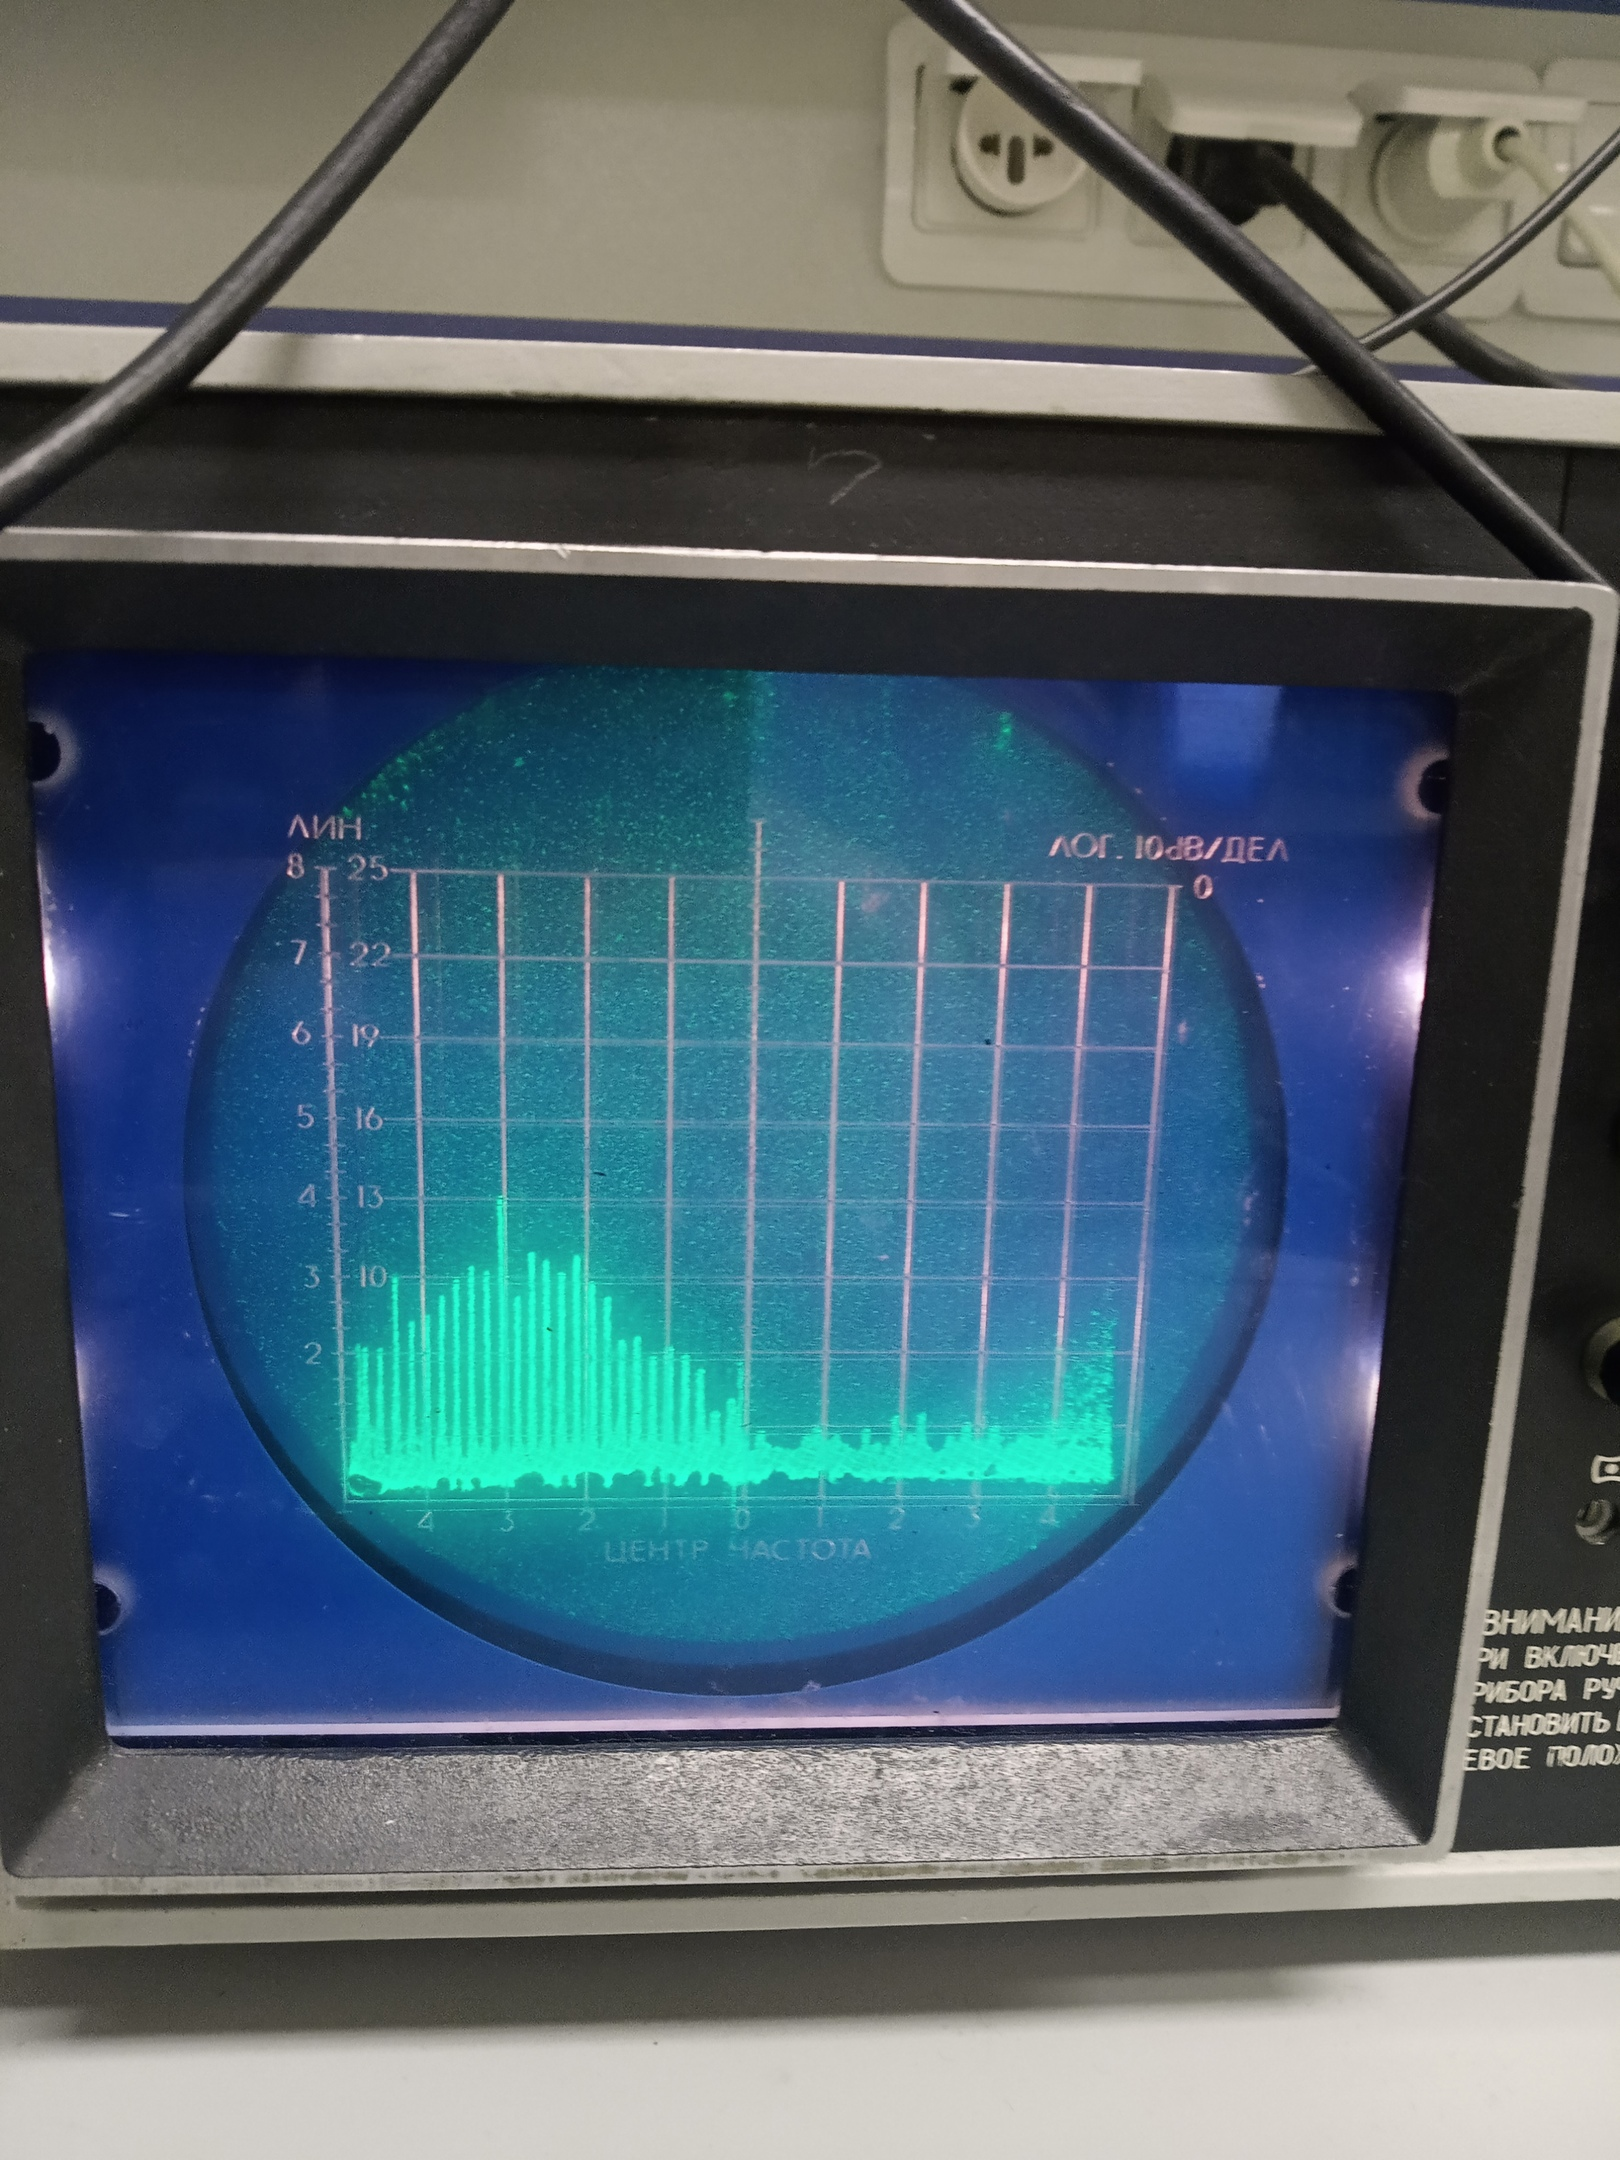
\includegraphics[scale=0.15]{sp6.jpg}
            \\\\
            \item $f_{повт} = 1 \text{ кГц, } \tau = 50 \text{ мкс, } \nu_0 = 40 \text{ кГц, }$
            
            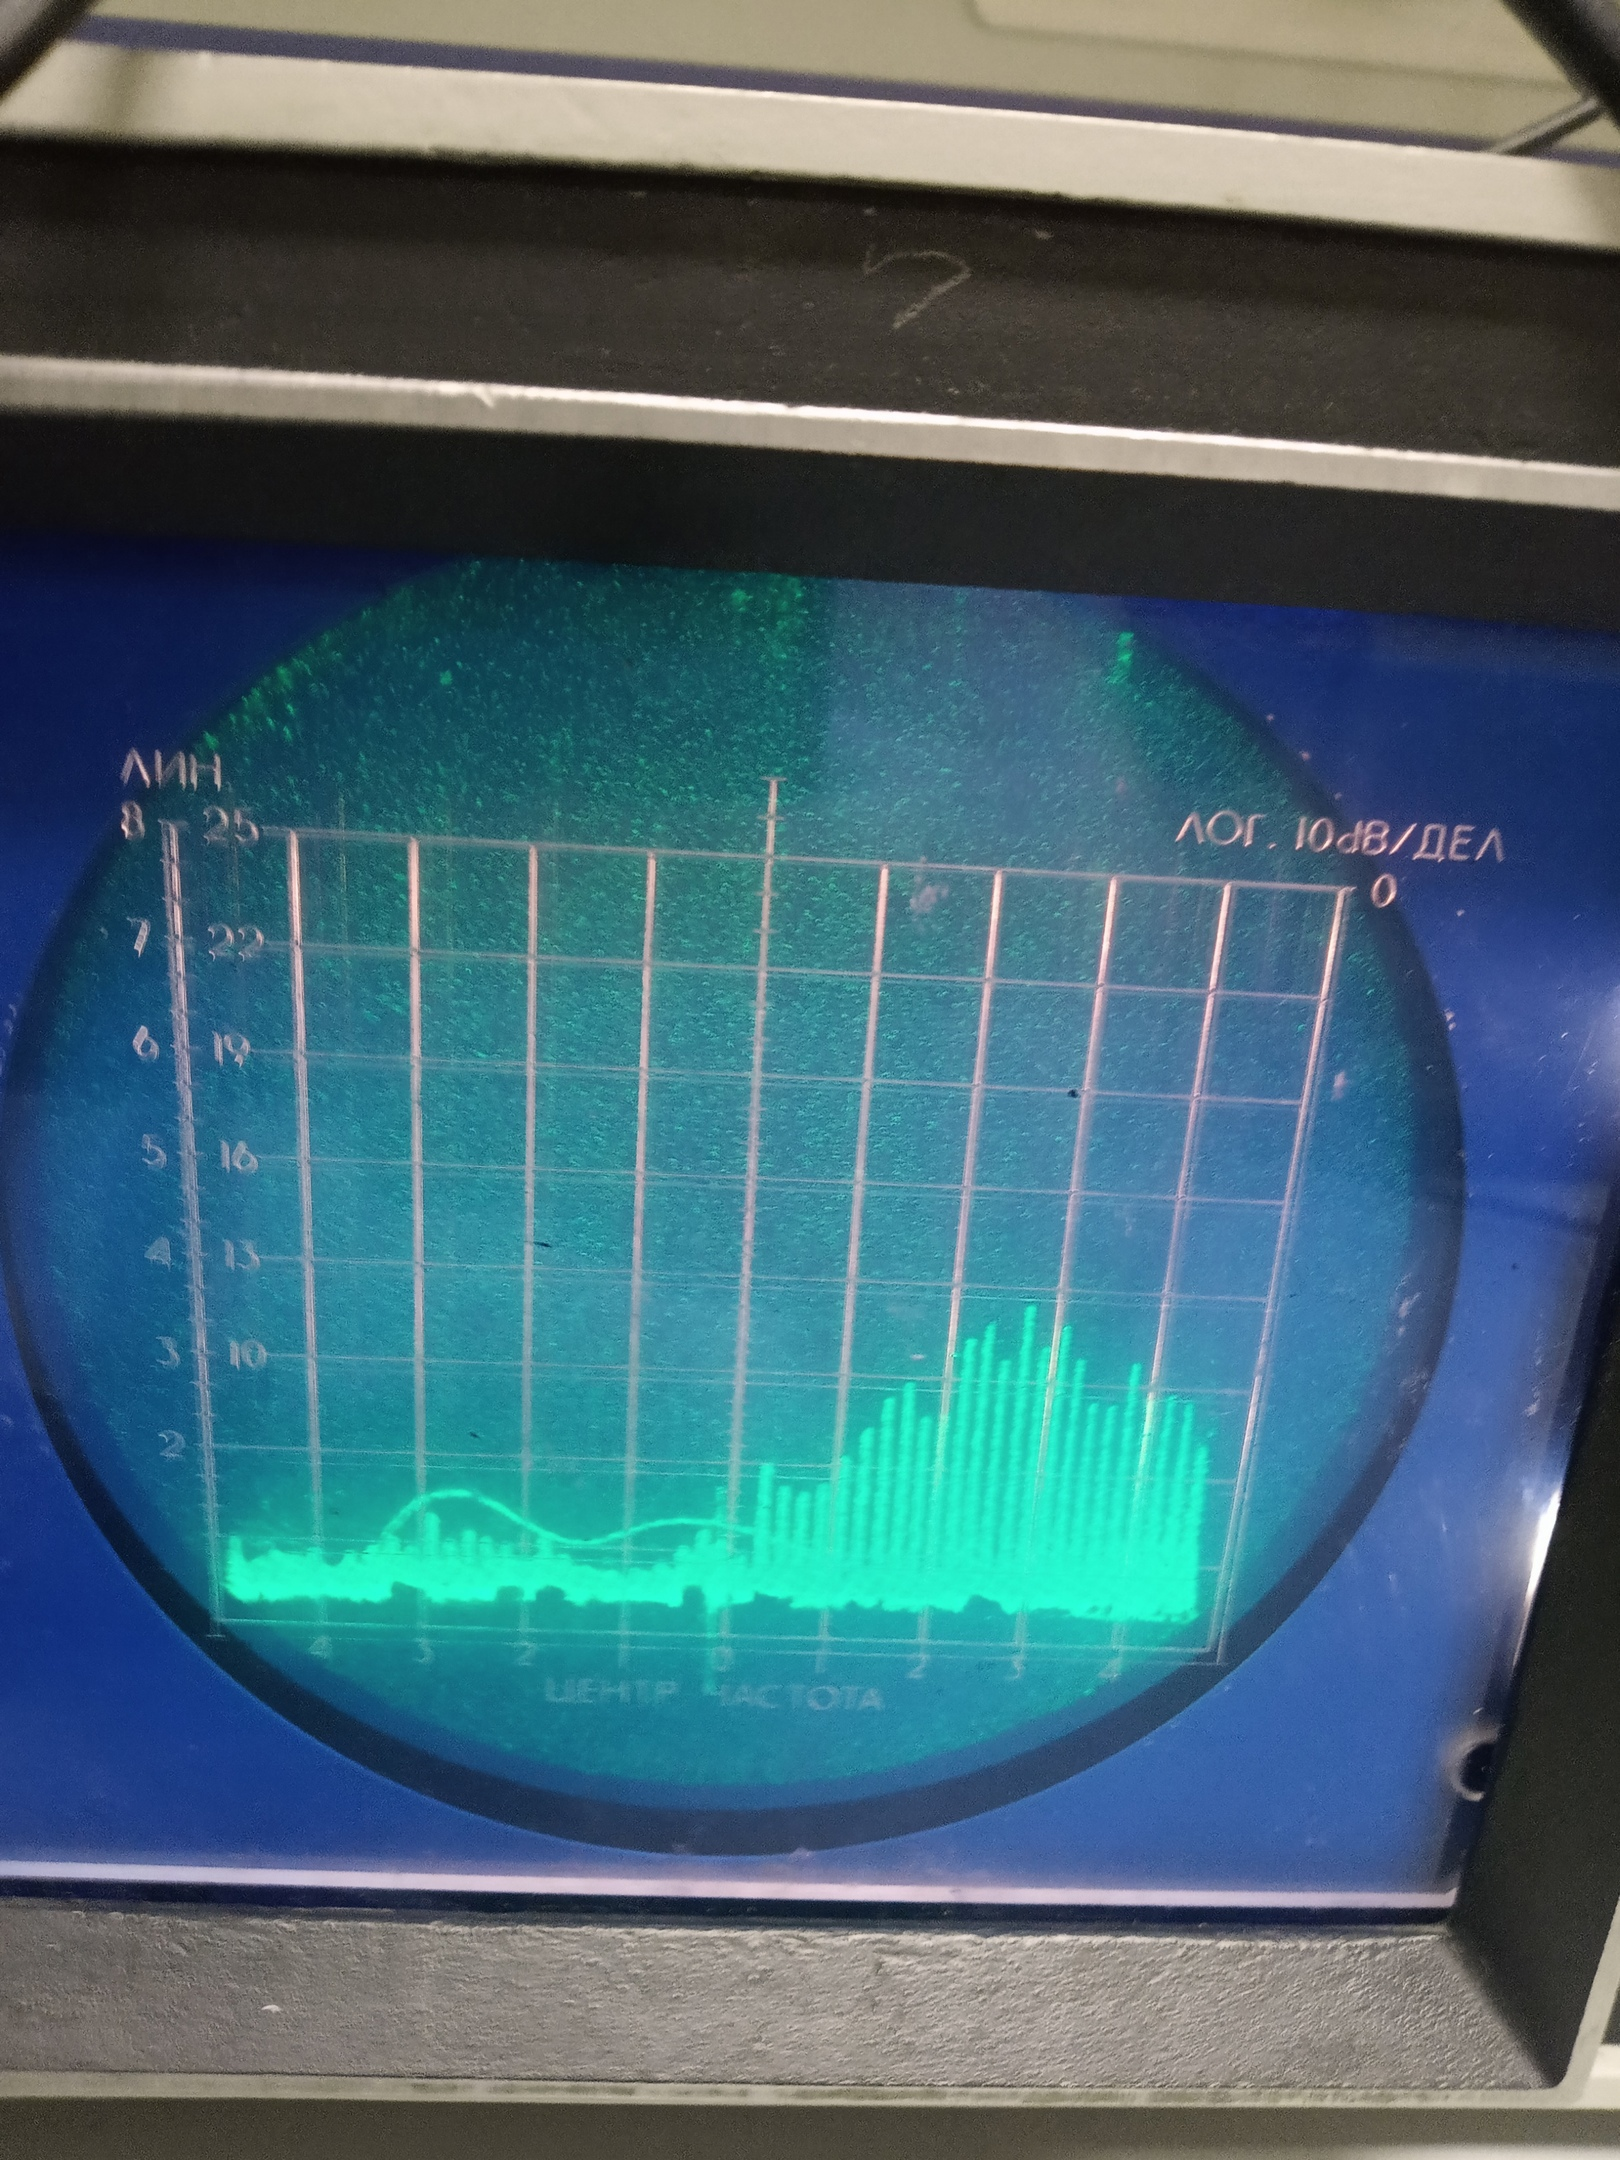
\includegraphics[scale=0.15]{sp7.jpg}
        \end{itemize}

        \item При фиксированной длине импульсов $\tau = 50$ мкс исследуем зависимость расстояния $\delta \nu$ между соседними спектральными компонентами от периода $T$ (частоты повторения импульсов $f_{повт}$ в диапазоне 1-7 кГц).
        
        \begin{tabular}{|c|c|c|c|c|c|c|c|} \hline
            $\delta \nu$, Гц & 555 & 2500 & 3333 & 5000 & 5000 & 6666 & 7500 \\ \hline
            $f_{повт}$б Гц & 1 & 2 & 3 & 4 & 5 & 6 & 7 \\ \hline
        \end{tabular}

        \item Построим график $\delta \nu \left( f_{повт}\right)$ (рис.~5)
        
    \end{enumerate}

    \mysec{В. Исследование спектра гармонических сигналов, модулированных по амплитуде}
    
    \paragraph*{Экспериментальная установка.} Схема для исследования амплитудно-модулированныого сигнала представлена на рис.~6. Модуляционный генератор встроен в левую часть генератора сигналов Г6-34. Синусоидоидальный сигнал с частотой модуляции $f_{мод} = 1$ кГц подается с модуляционного генератора на вход АМ (амплитудная модуляция) генератора, вырабатывающего синусоидоидальный сигнал высокой частоты. Амплитудно-модулированный сигнал с основного выхода генератора поступает на осциллограф и на анализатор спектра.

    \begin{figure}
        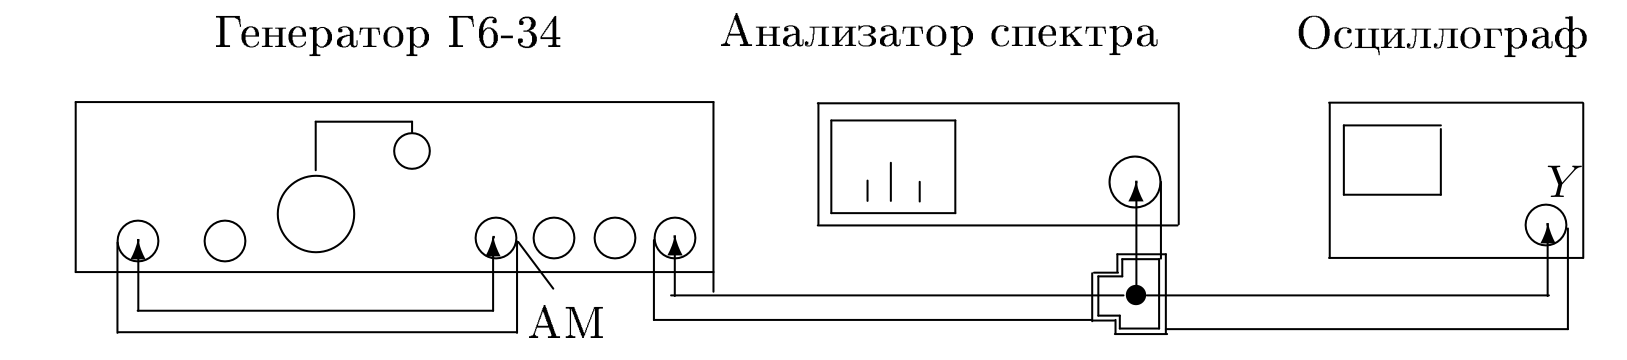
\includegraphics[scale=0.3]{pic4.png}
        \caption{Схема для исследования спектра высокочастотного гармонического сигнала, промодулированного по амплитуде низкочастотным гармоническим сигналом}
    \end{figure}

    \paragraph*{Задание.}

    \begin{enumerate}
        \item Соберем схему, изображенную на рис.~6.

        \item Исследуем зависимость отношения $a_{бок} / a_{осн}$ от $m = \frac{A_{max} - A_{min}}{A_{max} + A_{min}}$ ($A_{max}, A_{min}$~---~максимальная и минимальная амплитуда сигнала на осциллографе, $a_{бок}, a_{осн}$~---~амплитуда боковой линии спектра и основной линии спектра)

        \begin{tabular}{|c|c|c|c|c|c|c|} \hline
            $a_{бок} / a_{осн}$ & 0.0497 & 0.146 & 0.2329 & 0.3323 & 0.4317 & 0.4752 \\ \hline
            $A_{max}$ & 1.1 & 1.3 & 1.5 & 1.7 & 1.9 & 2 \\ \hline
            $A_{min}$ & 0.9 & 0.7 & 0.5 & 0.3 & 0.1 & 0 \\ \hline
        \end{tabular}

        \begin{figure}[!h]
            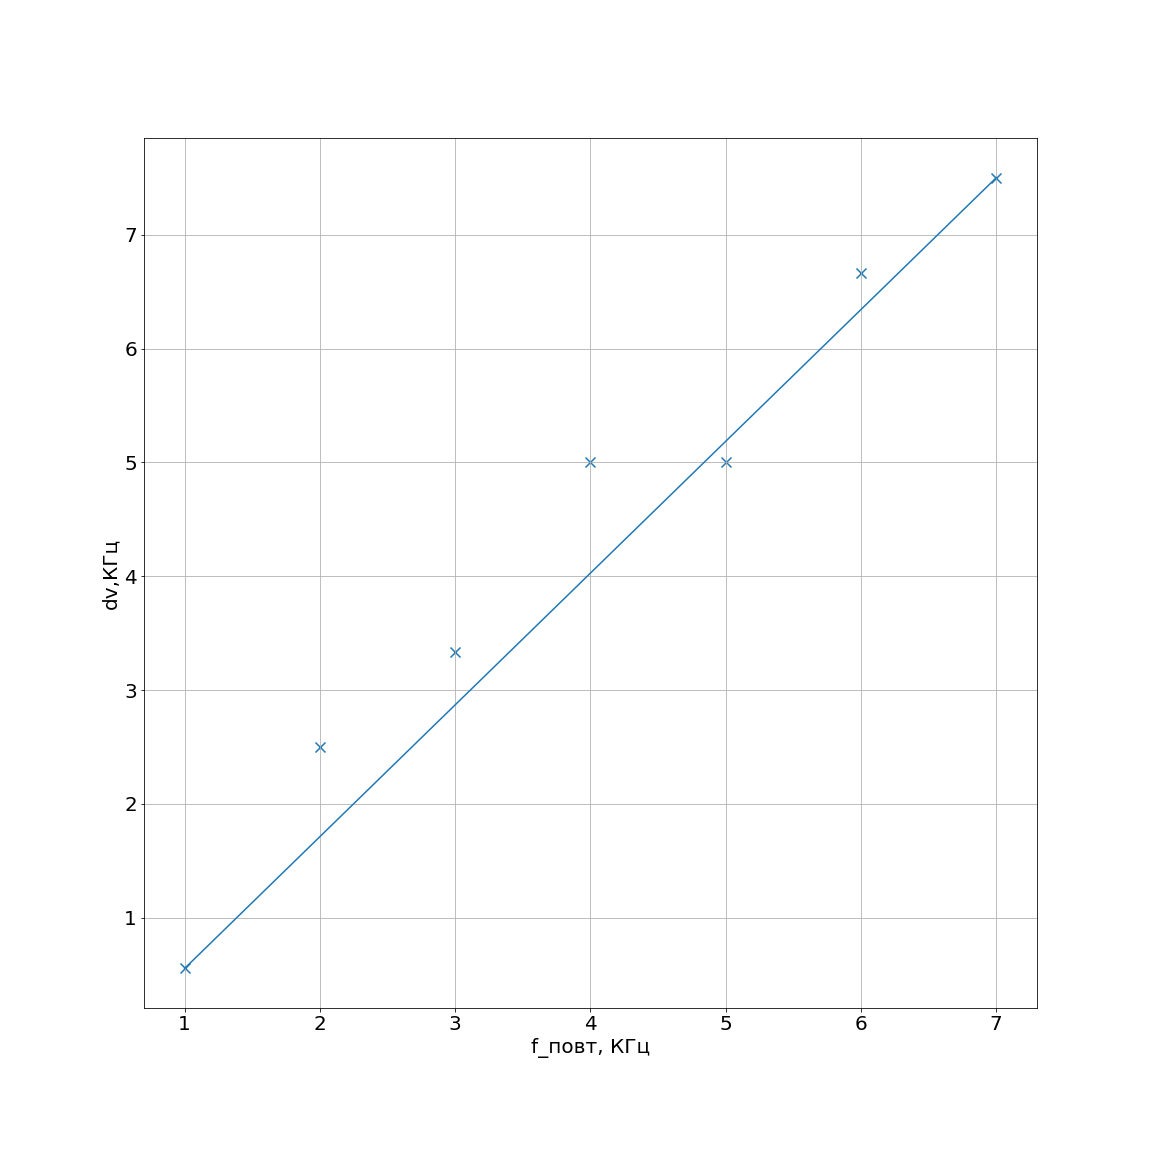
\includegraphics[scale=0.4]{graph2.png}
            \caption{График $\delta \nu \left( f_{повт}\right)$}
        \end{figure}

        \item Посторим график  $a_{бок} / a_{осн}$ от $m$
        
        \begin{figure}[!h]
            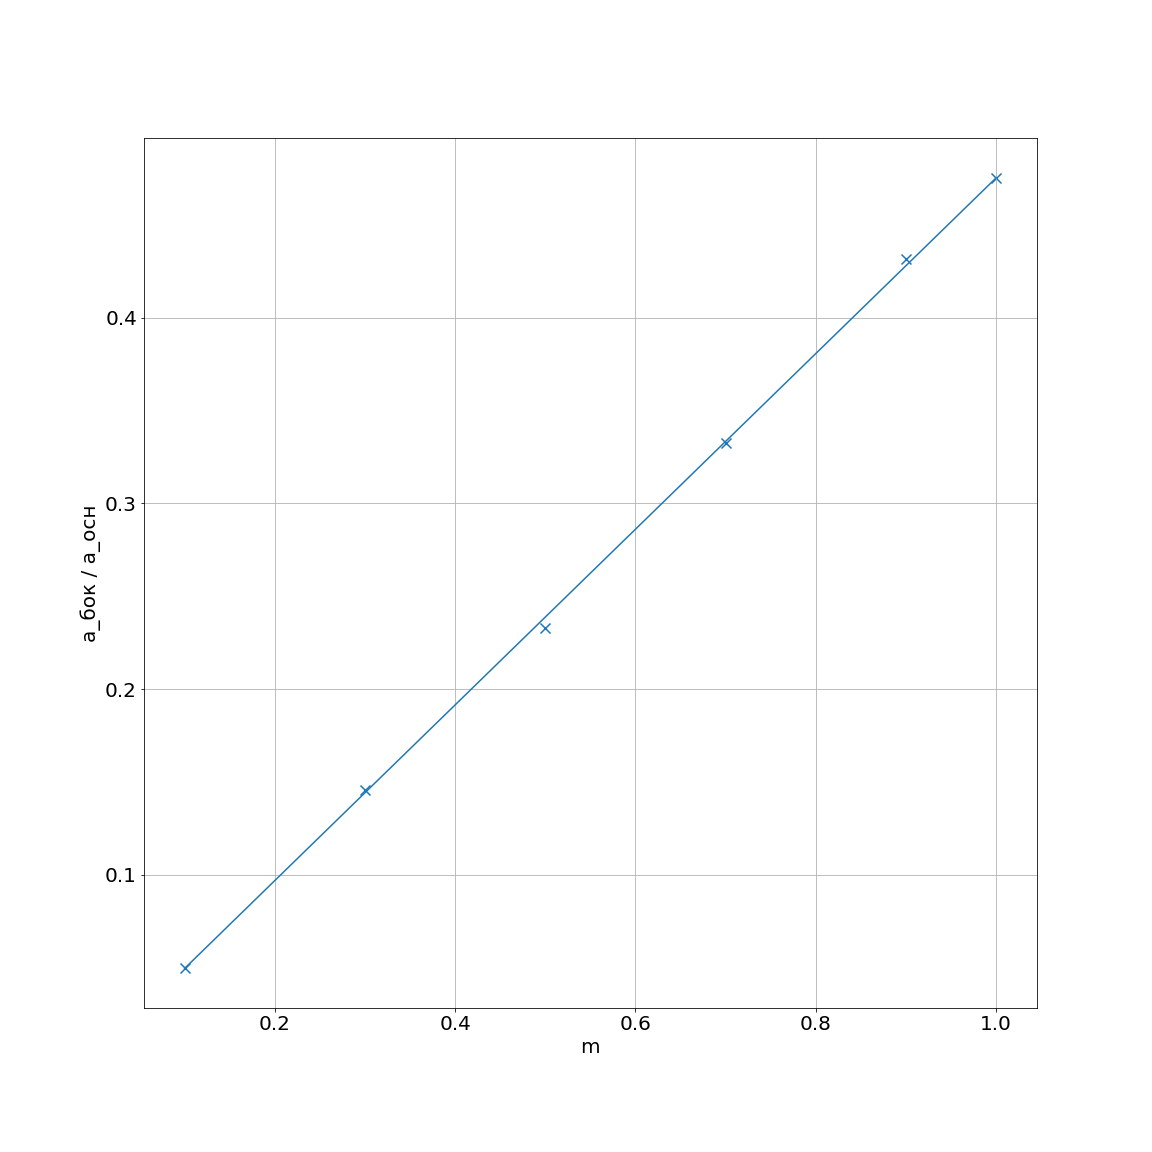
\includegraphics[scale=0.4]{graph3.png}
            \caption{График $a_{бок} / a_{осн}$ от $m$}
        \end{figure}

        \item Определим угол наклона графика:

        $\alpha_{граф} = \arctan{0.473} = 0.44$

        $\alpha_{теор} = \arctan{0.5}   = 0.46$
    \end{enumerate}
    
\end{document}